\section{Research Design}

After laying out the methodology used throughout the study, the actual application of the methodology has to be laid out. This is going to be the subject of this chapter. In the following considerations on research ethics, as well as participant selection are described. In addition to that, the development of the technology probes, the process for going through these probes, the technological setup for data collection, and the data analysis approach are documented in detail. The study approach as a whole is then summarized at the end of this chapter.

\subsection{Research Ethics}

Before delving into the specifics of the study an important, sometimes neglected, aspect of the study design has to be talked about: \textit{Research Ethics}. In order to do an ethically sound study with participants some important principles have to be met. Flick proposed eight principles of ethical research, that this study aims to follow (taken from Flick \cite[p. 135]{flick2018introduction}):

\small{
  \begin{enumerate}
    \item{\textit{Researchers have to be able to justify why research about their issue is necessary at all}}
    \item{\textit{Researchers must be able to explain what the aim of their research is and under which circumstances subjects participate in it}}
    \item{\textit{Researchers must be able to explicate the methodological procedures in their projects}}
    \item{\textit{Researchers must be able to estimate whether their research acts will have ethically relevant positive and negative consequences for the participants}}
    \item{\textit{The researchers must assess the possible violations and damages arising from doing their project}}
    \item{\textit{The researchers have to take steps to prevent violations and damages identified according to principle 5 above}}
    \item{\textit{The researchers must not make false statements about the usefulness of their research}}
    \item{\textit{The researchers have to respect the current regulations of data protection}}
  \end{enumerate}
}

To meet these requirements towards ethics participants have to be informed on each of the principles mentioned above. To achieve this, both a form of consent and a data protection information sheet have been created, that can be found in appendix \ref{append:consent}. Principles 1 through 3 should be met, by describing in the beginning paragraph and the subsections \textit{General Study Information} and \textit{Overall Study Procedure} of this form. Concerning principles 4 through 6, there should not be any positive or negative consequences for the participants, as the study only consists out of a virtual probe with questions only on the expertise of the participants, not on personal or intimate details. Should the participants wish to participate anonymously, an option is given as well. If the participants check this option in the online form, the gathered data is stored by using an random identifier number not connected to their name. As for principle 7 no false statements on the goals of the research are made, the goals match those mentioned within this thesis. Finally, the last principle is met by including all relevant information on the specifics of data processing in the subsection \textit{Confidentiality and Data Processing}. Therein everything that is logged is described together with where and how it is logged and processed. To make it clear for participants, that they can withdraw their participation in the study whenever they want, an additional section (\textit{Rights}) is added to the form. The resulting form is then presented to every participant before they start taking part in the probe and without consenting to it the probe cannot be started.

In addition to the considerations that are part of the consent, due to the current, ongoing COVID-19 pandemic there are additional considerations to be made. These mainly revolve around not requiring the participants to take part in a study on-site. As mentioned before, the probe is going to be done remotely, therefore, there is no need for additional precautions have to be taken on that account.

\subsection{From Theory to Probe}

The most important part of the research design arguably is the actual technology probe. As described in the methodology section, this requires careful attention to the features described by Hutchinson et al: \textit{Functionality, Usability, Logging, Flexibility, Design Phase} \cite[p. 499-500]{hutchinson2003technology}. The functionality is determined by the design implications found in literature and described in detail in the following chapter. Concerning the usability, Hutchinson et al. only state that there should not be any incremental changes during a probe, therefore this is not further elaborated on. Logging is going to be part of the data collection phase of the probe and therefore is described in the respective chapter. Finally, concerning the design phase, the probe is developed as the very start of the design process within this thesis but also as the start of further implications in this line of research.

A crucial part of developing the technology probe is the transition from theory to a finished probe to the execution of that probe. Therefore, this chapter is mainly concerned with the tasks done and decisions made in between those steps. At the start of this process is the transformation from the design implications and attributes of play discovered during literature research into actionable probe features. This again is divided into multiple sub-steps, the first of those steps being an ideation phase. Within that ideation phase, the design implications are used as a starting point based on which possible features, playful elements and game mechanics are ideated upon. This is loosely based upon IDEO's brainstorming principles \cite{ideo2021brainstorming}, as can be seen in \textit{Figure \ref{fig:probeideation}}.

\begin{figure}[h]
  \centering
  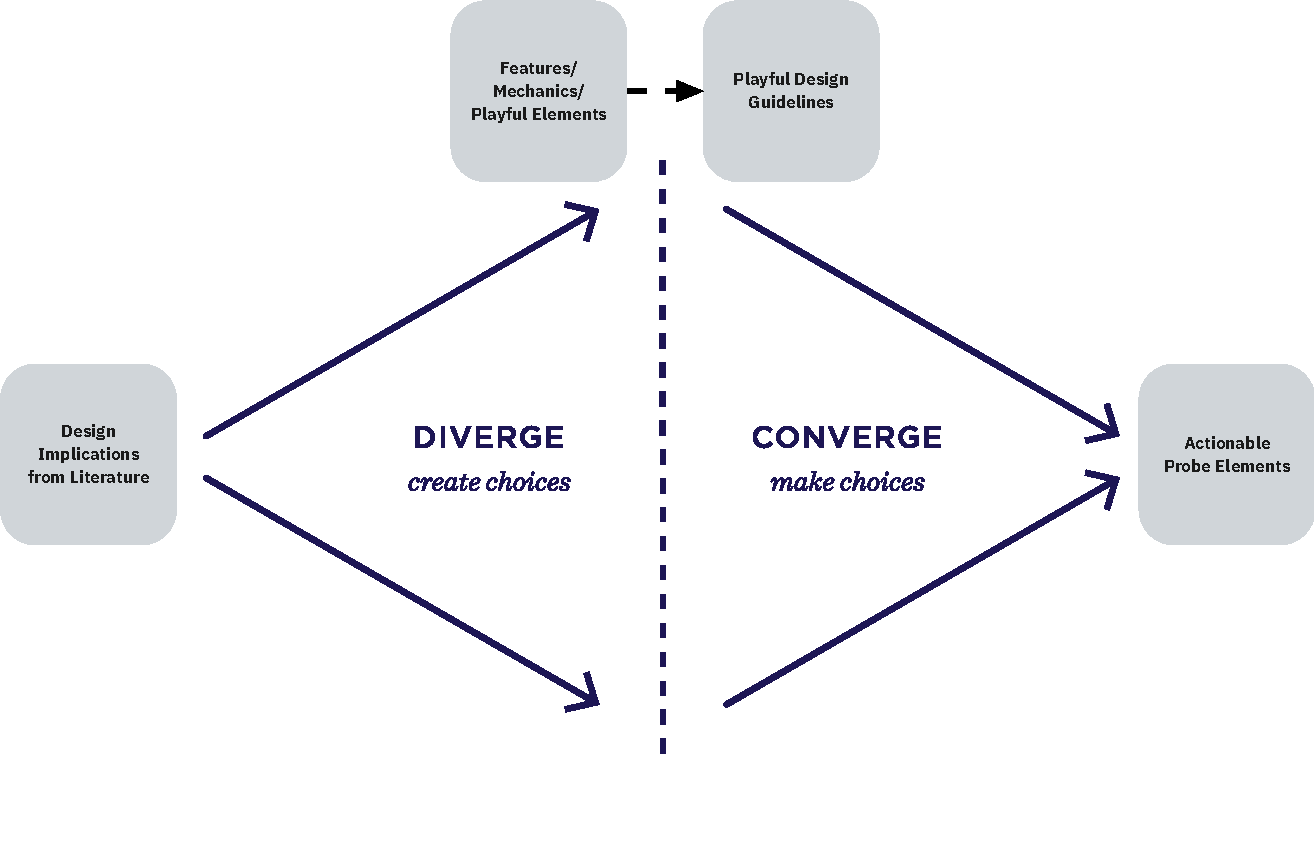
\includegraphics[width=\textwidth]{probeideation.pdf}
  \caption{Adapted IDEO Brainstorming Process (originally by IDEO U \cite{ideo2021brainstorming})}
  \label{fig:probeideation}
\end{figure}

Starting with the design implications as much features/concepts/playful elements as possible are ideated upon to generate a variety of technological choices as possible rooted in literature. With those generated, the next step then is to \textit{make choices}, meaning, deciding on a few that then can be implemented within the technology probe. Concerning this thesis, the respective brainstorming process is visualized and documented in \textit{Appendix \ref{append:probe-design}}. Therein you can see the implications on the far left of the diagram, based on these a braindumping session \cite{ia2021dumping} was held. The result of this session is visualized to the right of the attributes of play within \textit{Appendix \ref{append:probe-design}}. Examples of the ideas gathered are:

\begin{itemize}
  \item{Serendipitous random effects within the game/probe}
  \item{Generate game objects for contributions and possible tasks}
  \item{A Stage where the players can explore for themselves}
\end{itemize}

For the full list, refer to the respective diagram in the appendix. What is also shown in this diagram, is on what kind of design implication the respective idea is based upon. These ideas were then condensed into actual guidelines that can inform the probe implementation or any kind of playful design for that matter. After that converging these guidelines is necessary. This is done for two reasons. One, to reduce the number of features in order to conform to the technology probe attribute of \textit{functionality} described by Hutchinson et al. \cite[p. 18]{hutchinson2003technology}. Two, in order to create actionable tasks rather from the very vague ideas and slightly less vague guidelines. The results of this process can be seen in detail in \textit{Appendix \ref{append:probe-design}}. The converging itself was done by combining and reducing the guidelines so that an implementable task description is reached. If some guidelines were not included as features, these were dismissed by me based on the perceived difficulty of implementation. That is because the technology probe should be kept simple and focused on gathering as much valuable data as possible rather than being an intricate and detailed prototype implementation.

Another important decision to be made at this point is which onboarding level the probe should focus on. Should it be on the source code/programmatic level, should it be at the process level or should it be at a social \& developer-centered level. This decision depends on a few things. At first, it has to work in a remote, decentralized settings due to the constraints defined in the previous chapter. Secondly, it has to be \enquote*{implementable} by me, based on the timeframe and my previous experience. Thirdly, and arguably most importantly, the probe should be able to collect data, that contributes and extends this line of research. Concerning this third statement, there is no actual constraint imposed by existing research, as on none of the described onboarding levels, there are existing implementations in research. The first and second statement on the other hand do impose some constraints. Because of the remote setting, a social setting might be hard to replicate remotely. In addition to that, as is going to be described in chapter 4.5, the study is not going to be done within one single team of developers working on one project, rather the probe is targeted towards individual developers. This further increases difficulty in deploying a probe within a social setting. Therefore the probe is rather going to focus on program comprehension and process-centered techniques like information seeking and feature location, which can be implemented on a source code/project level. Nonetheless, research into the other levels of onboarding could be equally valuable in the future.

At this point most of the non-technical decisions have been made. From the design implications, an ideation phase, followed by a phase of converging, produced a set of possible features that can be implemented. As mentioned before, these are shown in the second-to-last column in \textit{Appendix \ref{append:probe-design}}. Actually deciding on the feature set used in the probe, depends on some technical decisions, though. This is why in the follwoing chapter there is going to be a deep-dive into all technological considerations including the final feature set.

\subsection{Probe Implementation}

To actually implement a coherent technology probe, these considerations have to be discussed in detail, starting with the choice of technology in which to implement the probe. As described in the previous chapter, the probe is going to target the psychology- and process-centered level of onboarding and is based on the source code and meta-information of a project. Best-case this probe could be applied to any project independently from its technology. Depending on the programming language and framework there are grave differences in project structure, though. A \textit{Ruby on Rails} \footnote{\url{https://rubyonrails.org/}, accessed on 10th of August 2021} project for example, gives the developer a fixed structure out of the box, while there is no such structure when developing a \textit{node.js} \footnote{\url{https://nodejs.org/en/}, accessed on 11th of August 2021}, project with \textit{express.js} \footnote{\url{https://expressjs.com/}, accessed on 11th of August 2021}. Creating a probe that would work with both of those examples, or even more than that, would not be feasible in the given timeframe. More importantly, for a probe meant to be executed once by each participant, there is no benefit in investing additional implementation time into allowing the probe to work on multiple, differently structured projects in succession. More specifically, in the case of this probe the underlying project is not going to be changed for each participant to achieve some amount of comparability between the experiences of the developers. Deciding on which specific project to choose depends on some constraints as well, though.

First of all in order to build a probe, that can be sent out to developers not necessarily working within the same company and/or team, the source code has to be publicly accessible. This rules out projects proprietary to a single company or team right away. In addition to that the project should cater to the knowledge of a wide variety of developers. Therefore, the technology used within the project underlying the probe should be popular enough, that a general understanding of the project setup is possible for the participants. According to a survey done by StackOverflow Insights \footnote{\url{https://insights.stackoverflow.com/}, accessed on 11th of August 2021} with 83,052 responses on the topic of programming languages developers have done extensive development in the last year, there is a clear leader in popularity (multiple responses by developers were possible): \textit{Javascript} (64.96\% agreement), its server-side framework \textit{node.js} (33.91\% agreement) and its superset \textit{Typescript} (30.19\% agreement), with the closes other technology/programming language being \textit{Python} (48.24\% agreement) \cite{so2021}. Thus, choosing a \textit{Javascript, node.js} or \textit{Typescript} project, might be the most approachable for a wide variety of developers. The only downside to choosing such a project, is that none of these technologies by themselves give a fixed structure to rely on when building a probe upon it. Something that gives that structure, is the concept of monorepos.

These are repositories, where the \enquote{codebase is contained in a single repo encompassing multiple projects} \cite[p. 226]{jaspan2018advantages}. This gives inherent structure to the project, with different subprojects as a whole to explore on different levels. Also, larger codebases might profit more from onboarding help due to the increased complexity going hand in hand with the increase in size. Moreover, in a well-crafted monorepo, any \enquote{ project in the repo can be built only from dependencies also checked into the repo} \cite[p. 226]{jaspan2018advantages}. This allows for visualizations of these connections within the monorepo and how subprojects realte to each other. Especially so, when combined with \textit{Javascript}-based monorepo-organization tools like \textit{Lerna} \footnote{\url{https://lerna.js.org/}, accessed on 11th of August}. \textit{Lerna} stores information on the dependencies within the monorepo in two files, \verb|package.json| and \verb|lerna.json|. In addition to that the subprojects are guaranteed to be found in a \verb|/packages| directory. This further allows for reading these files and directories in code in order to easily implement probe features on top. Consequently, a \text{Javascript/Typescript}-based monorepo that uses \textit{Lerna} or a similar tool, with predefined structure, where also the source code is publicly available has to be found. Fortunately, the largest provider of publicly available repositories, \textit{Github} \footnote{\url{https://github.com/}, accessed on 12th of August 2021} makes it possible to filter for these criteria (filter results can be found here \footnote{\url{https://github.com/topics/monorepo?l=typescript}, accessed on 12th of August 2021}). A highly popular monorepo, that is well maintained and actively collaborated on, is the \textit{ethereumjs-monorepo}, a repository containing the \textit{Javascript} implementation of the \textit{Ethereum} blockchain \footnote{\url{https://ethereum.org/en/}, accessed on 12th of August}. While this repository does not use \textit{Lerna}, it still follows the structure imposed by \textit{Lerna}, making it possible to programmatically read the monorepo information from its directories and \verb|package.json| file(s). Because of that and the repository matching the other constraints imposed on this decision, the \textit{ethereumjs} monorepo is chosen as the underlying project for the implementation of the technology probe.

The next decision to make is then the one of with which technology and in which in environment to create the technology probe. Due to the setting as a remote probe, the technology used for the probe should be easy to distribute to the participants, without any additional setup work on the researcher's, but also on the participant's side. The perhaps easiest way to achieve this, is to create an interactive web page, accessible through just an browser without any additional installation steps required. The downside of this approach would be, that the probe is removed from how most developers interact with the source code of a project -- through an \gls{ide}, text editor or the command line. Due to multiple editors and \gls{ide}s existing, there would have to be a decision for a single tool. This in turn limits the number of developers being able to take part in such a probe or doing so in an environment different from what they are used to. In addition to that different editors and \gls{ide}s use different plugin systems, for which a non-negligible amount of previous experience or time invested is required in order to develop plugins. This, together with my extensive experience in a web environment and with web technologies led to the decision of implementing the probe in a web environment.

Based on these decisions, the final feature set can ultimately be defined. Referring back to Hutchinson et al.'s probe features, a further reduction of features is in order. Therefore, special attention is paid to decide on a set of playful features, that can be transformed into a coherent probe not overflowing with too much functionality and with definitive boundaries. What also went into consideration, was an attempt to match probe features with concepts from the underlying project, to foster it being used as an educational tool -- similar to how Ian Bogost defined them \cite{bogost2007persuasive}. This led to the implementation of the following features:

\begin{itemize}
  \item{\textbf{Visualizing the overall project structure} -- Based on the idea that the code structure should be documented \cite[p. 10]{steinmacher2018let} and that the micro and macro structure of projects should be visualized \cite[p. 284]{dagenais2010moving}, as well as Sicart's notion of visualizing creative appropriations of data \cite[p. 28]{sicart2014play}}
  \item{\textbf{Free exploration within subprojects} -- Based on the idea that playful objects should be freely interacted with (based on Sicart's notion in \textit{Play Matters} \cite[p. 40]{sicart2014play}) and the idea that players should explore and test without too much guidance (based on Sicart's notion in \textit{Play Matters} \cite[p. 57]{sicart2014play})}
  \item{\textbf{Implementation of a reveal mechanic to uncover objects in subprojects} -- Based on the idea that users should complete intentionally ambigious designs (based on Sicart's notion in \textit{Play Matters} \cite[p. 31]{sicart2014play}) and the idea that uncertain outcomes should be embraced, where the user can decide (based on Rodriguez as described in chapter 2.4 \cite{rodriguez2006playful})}
  \item{\textbf{Discovery of potential issues} -- Based on the idea, that specific tasks should be recommended to the newcomers in a project (based on \cite{latoza2006maintaining}, \cite[p. 36]{yates2014onboarding}, and \cite[p. 8]{steinmacher2018let})}
  \item{\textbf{Discovery of important contributors} -- Based on the idea, that social links in development projects are crucial and mentors should be recommended to newcomers (based on \cite[p. 8]{steinmacher2018let} and \cite[p. 284]{dagenais2010moving})}
  \item{\textbf{Discovery of 3rd-party packages used} -- Also based on the idea of visualizing the micro and macro structure of a project \cite[p. 284]{dagenais2010moving}, where 3rd-party packages are part of both the code (=micro) and the overall structure (=macro) depending on the package}
  \item{\textbf{Creation of a companion helper} -- Based on the idea, that a companion with personality enables playfulness (based on Sicart's notion in \textit{Play Matters} \cite[p. 32]{sicart2014play}}
\end{itemize}

These features can be combined into a coherent \textit{game world}, that visualizes the project structure, but also enables the players to playfully explore specific parts of the project. While the companion feature deviates from this coherent set, it nonetheless can be implemented as a tool of communication and occasional helper for the other features. Overall this should allow the technology probe to be succinct enough in functionality (again referring to Hutchinson et al. \cite[p. 18]{hutchinson2003technology}) while also being open-ended (as mentioned by Hutchinson et al. as well \cite[p. 19]{hutchinson2003technology}) enough in paths towards the exploration.

With that decided upon, the actual implementation now can commence. This implementation can be split into two distinct parts. Firstly, the generation of the \textit{game world}, and the discoverable elements of the probe from the underlying project. Secondly, the actual implementation of the user-facing, interactive part. These are described in detail as follows, starting with the user-facing implementation as the generation of the game world is based on how it should be visualized in the end.

\subsubsection{The User-Facing Implementation}

First of all a general idea of how the probe should be visualized aesthetically. Aesthetics play a vital role in the creation of any kind of probe. Gaver et al. point out, that they \enquote{believe aesthetics to be an integral part of functionality} \cite[p. 25]{gaver1999design}. Gaver et al. also mention, that a finish that is too professional could lead to the probe being perceived as too formal \cite{gaver1999design}.

Thus, a balance between appealing aesthetics and a simple but functional visualization has to be found. To find this balance, several examples of a minimal but functional aesthetic were collected in order to create a rough direction forward in terms of visual design of the probe. These examples can be found in \textit{Figure \ref{fig:probeinspiration}}. All of these have in common, that they are so-called \textit{Minimalist Game Designs}, which in addition to some other characteristics, are defined through \enquote{abstract audiovisual representations} \cite[p. 38]{nealen2011towards}. The characteristics of such games match the characteristics of technologies very well, as Nealen et al. point out, \enquote{these games feature a small set of mechanics and one core mechanic, while still being sufficiently deep and allowing for player exploration} \cite[p. 38]{nealen2011towards}. This suggests, that going for such minimal aesthetics might emphasize what the technology probe in itself is trying to achieve.

\begin{figure}[h]
  \centering
  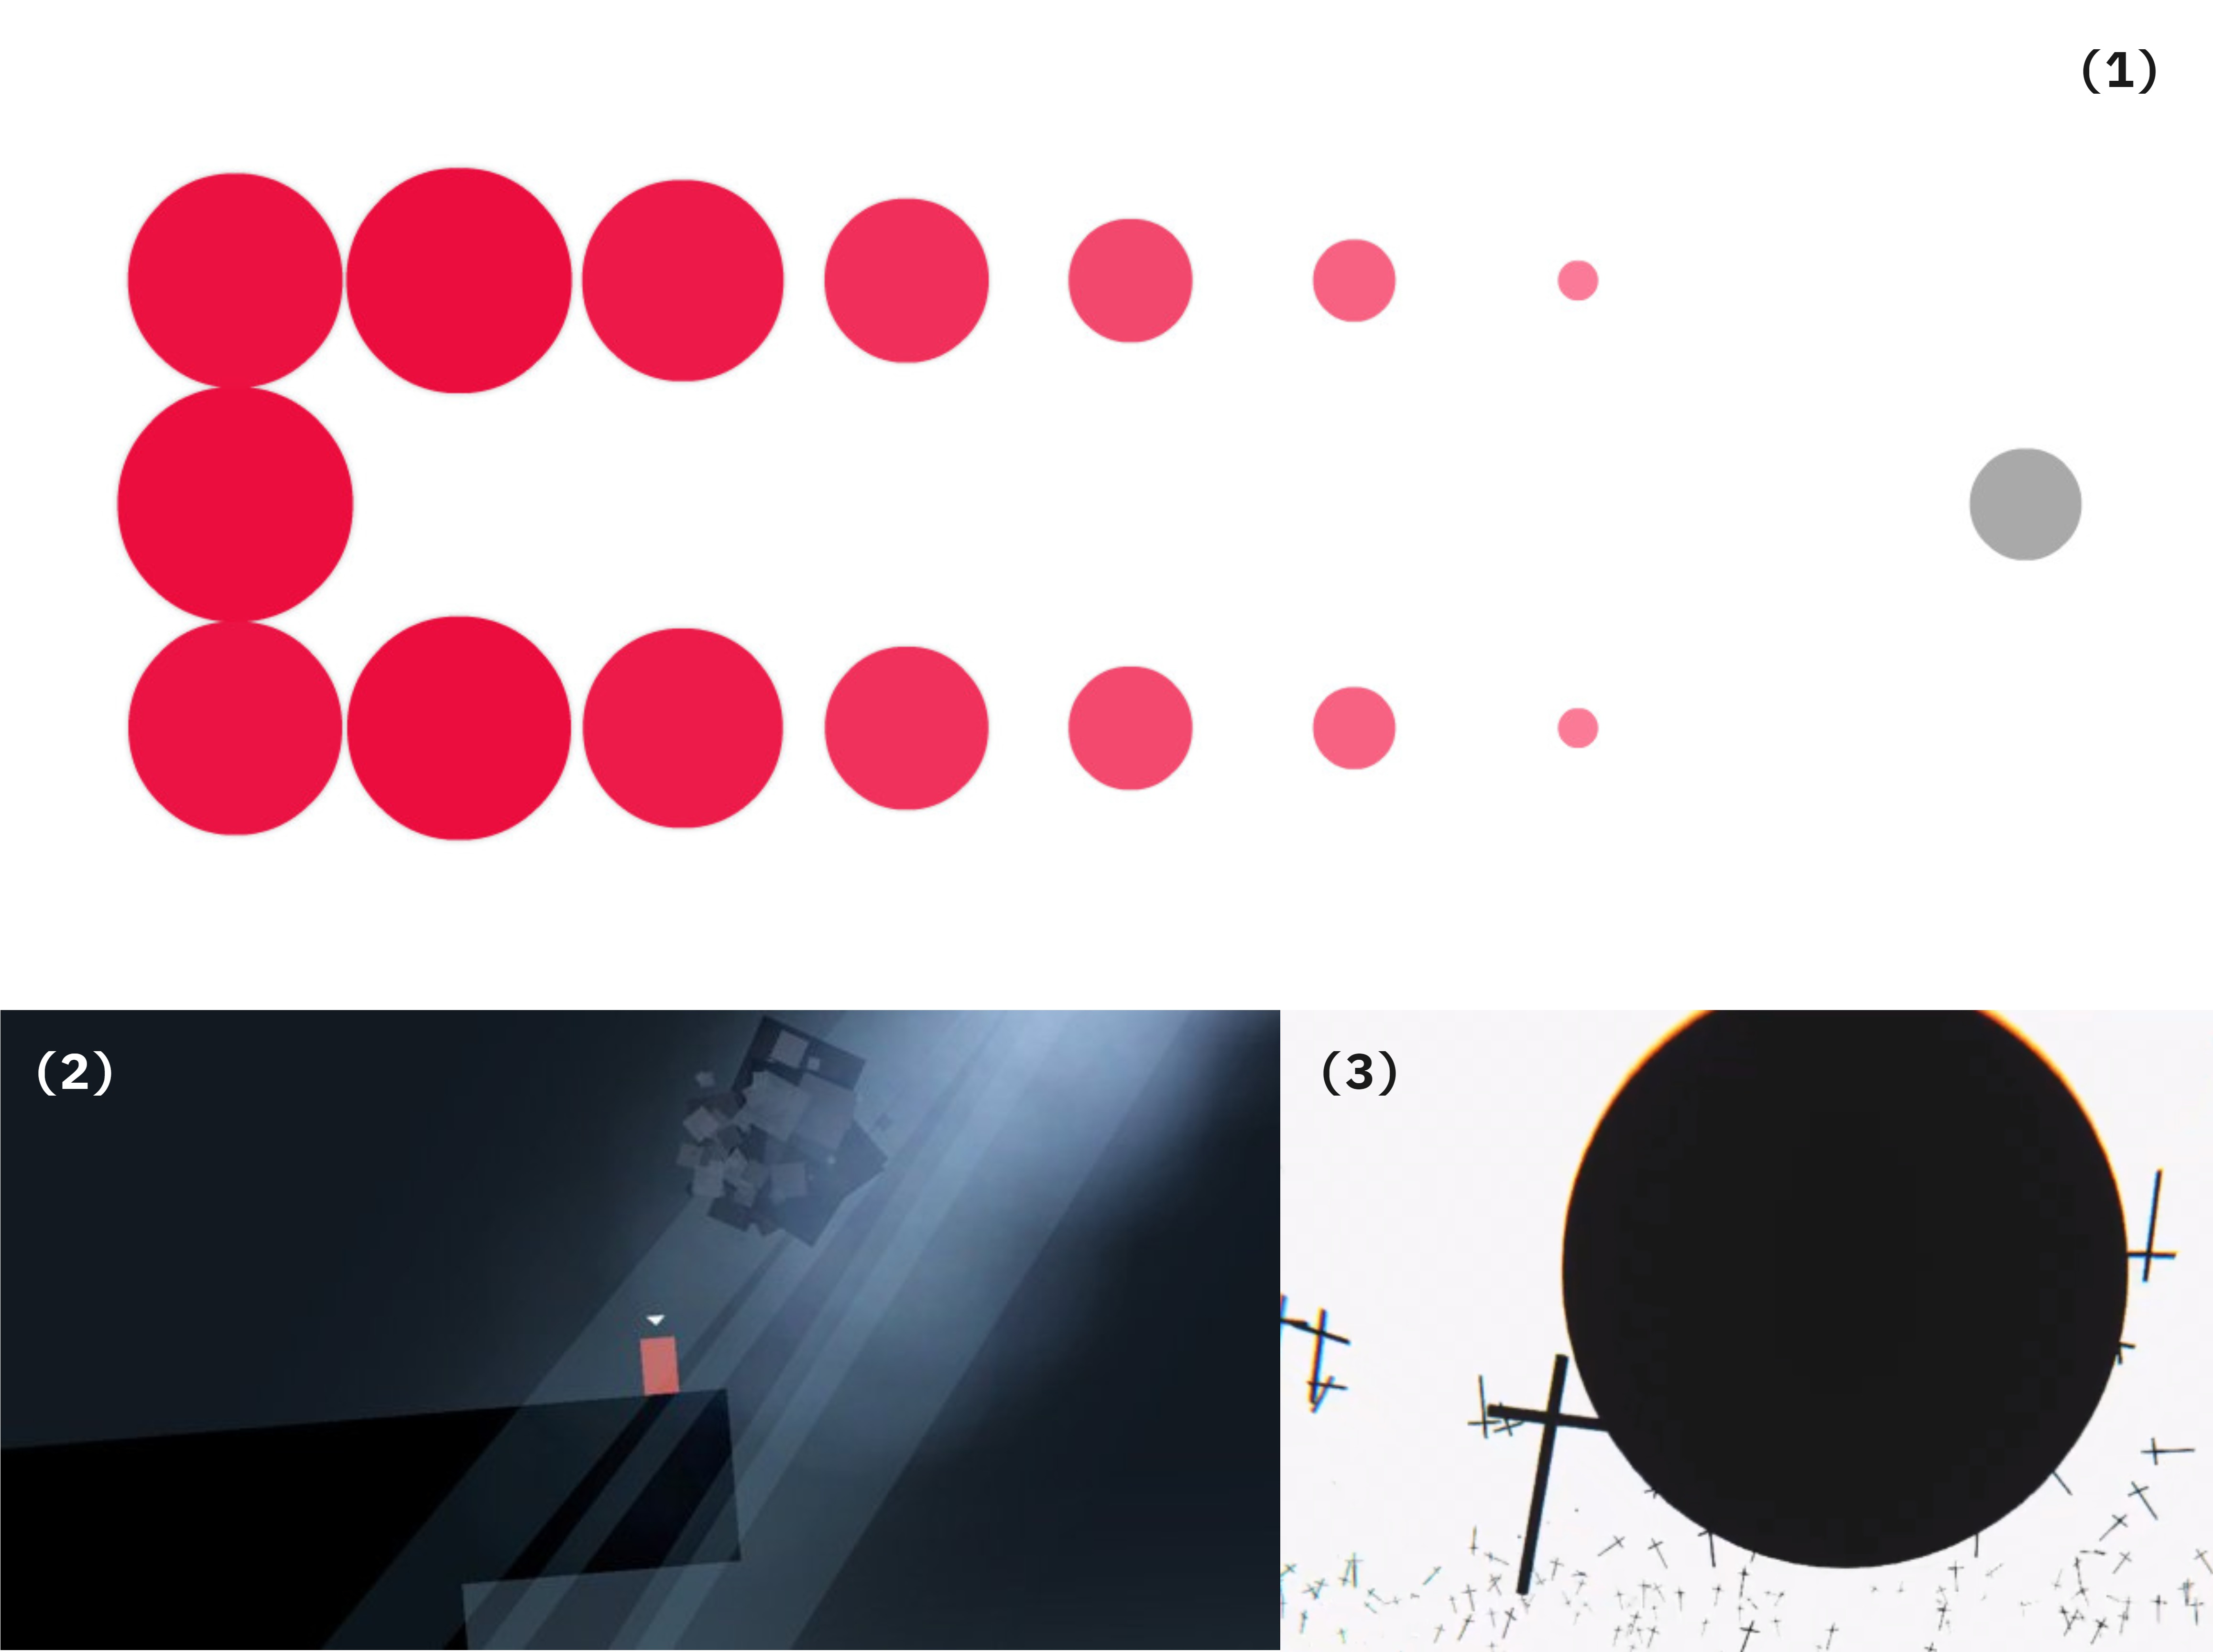
\includegraphics[width=\textwidth]{probeinspiration.jpg}
  \caption{Probe aesthetics inspiration (including \textit{Circles} \cite{circles2017} by Jeroen Wimmers (1), \textit{Thomas Was Alone} \cite{thomas2015} by Mike Bithell (2), and \textit{Carthasis} \cite{dribble2021} by Oleg Frolov (3))}
  \label{fig:probeinspiration}
\end{figure}

With the general aesthetic direction decided on, the next step revolves around developing a world within which the probe features can be implemented. This game world consists of the game objects representing the different, discoverable objects, a character the player controls, and the background setting. The background setting is going to be kept as minimal as possible, in order to achieve the goal of a minimal, ambiguous but explorable setting for the player. The overall color scheme should strengthen these goals as well, therefore a monochrome color palette, with only shades of red as the accent color used throughout the probe. Concerning how the actual objects within the game world look, these are also visualized as simple as possible, similar to how \textit{Circles} \cite{circles2017} is built. Rather than creating a visually intricate design, the playfulness comes from the interaction and from how the objects behave. All of the objects within the game world and their designs can be seen in \textit{Figure \ref{fig:probeobjects}}.

\begin{figure}[h]
  \centering
  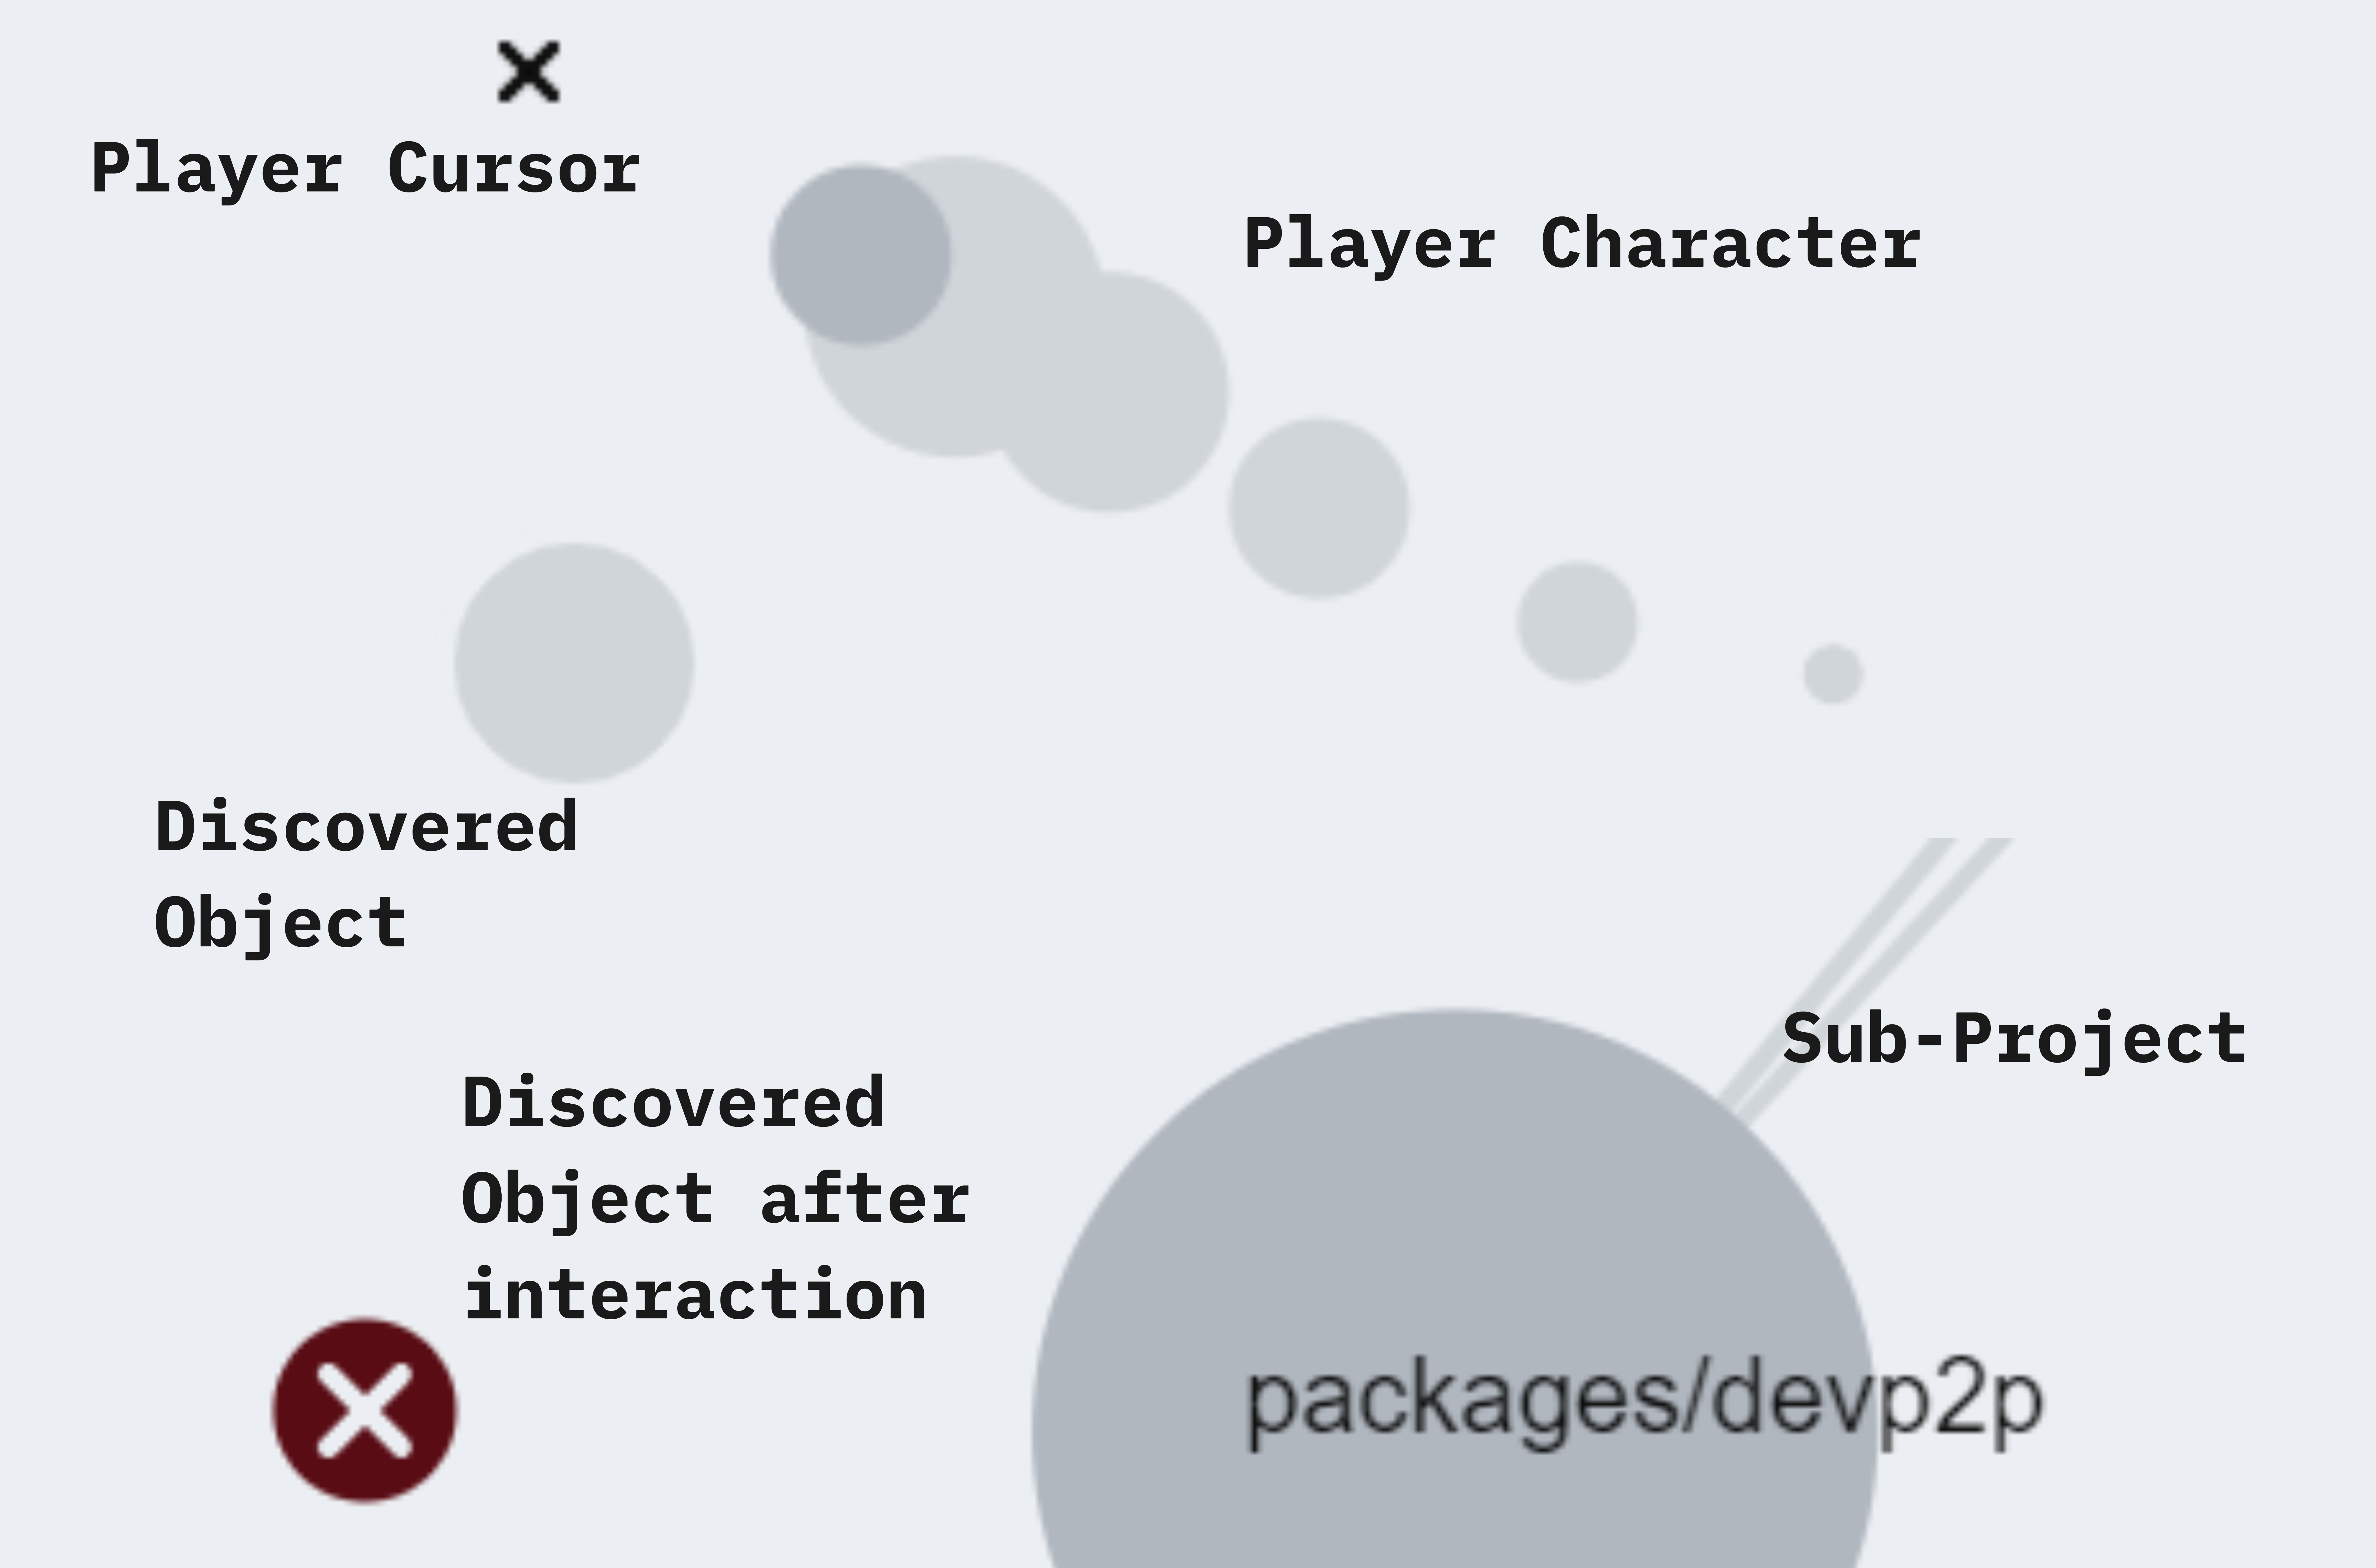
\includegraphics[width=\textwidth]{probelements.jpg}
  \caption{Game objects used throughout the technology probe}
  \label{fig:probeobjects}
\end{figure}

With the main game objects, the color scheme, the overall aesthetic direction and the features out of the way, the actual implementation can be undertaken at this point. In order to do this, the technical foundation has to be decided on. As mentioned before, the probe is going to be implemented as a web page, therefore the technology choice is limited to that space. Nonetheless, there is a huge variety of possible frameworks in that technology space to choose from. From entire game engines \& frameworks to using no framework at all and relying on \textit{Javascript, \gls{html},} and \textit{\gls{css}} alone. Using no framework at all -- especially when implementing a highly graphical and interactive application -- presents the need to re-implement a lot of features frameworks provide, like easy interaction handling, animation support and more. On the other hand a complete game engine brings much more, than is needed in this case. Due to the minimalistic visualization, there is no need for complicated physics replication or support for intricately designed sprites. A framework that sits in between those two extremes, is \textit{p5.js} \footnote{\url{https://p5js.org/}, accessed on 12th of August 2021}, a \textit{Javascript} implementation of the popular \textit{Processing} \footnote{\url{https://processing.org/}, accessed on 12th of August 2021} framework. It excels in creating interactive visualizations, especially when based on geometric shapes. Combined with my previous experience using this framework, it presents a suitable choice for the implementation of the technology probe. In addition to that there are more libraries used for different parts of the implementation to speed up the development. As a build tool, that helps bundling and transforming the written source code into a browser-compatible package and allows usage of \textit{Typescript} \footnote{\url{https://www.typescriptlang.org/}, accessed on 13th of August 2021}, \textit{Parcel} is used \footnote{\url{https://parceljs.org/}, accessed on 13th of August 2021}. To speed up development of all styling not connected to \textit{p5.js}, \textit{SASS} \footnote{\url{https://sass-lang.com/}, accessed on 13th of August 2021} is used. In order to use a central data store, that houses and distributes the current game state, the libraries \textit{Rx.js} \footnote{\url{https://rxjs.dev/}, accessed on 13th of August 2021} and \textit{zustand} \footnote{\url{https://github.com/pmndrs/zustand}, accessed on 13th of August 2021} are used. Other important helper libraries, include \textit{anime.js} \footnote{\url{https://animejs.com/}, accessed on 13th of August 2021} for animations outside of the interactive visualization, \textit{Moment} \footnote{\url{https://momentjs.com/}, accessed on 13th of August 2021} for date manipulation, \textit{Lodash} \footnote{\url{https://lodash.com/}, accessed on 13th of August 2021} for general utility functions and \textit{Firebase} \footnote{\url{https://firebase.google.com/}, accessed on 13th of august 2021} as a way to persist logging information and answers to the questions accompanying the probe. For the full list of all 3rd-party packages used throughout the probe, refer to the \verb|package.json| \footnote{See suppl. repository at path: \texttt{./technology-probe/package.json}} within the repository, where the probe's source code is managed.

All of these technologies serve the goal of creating the technology probe in the end. This creation itself can be divided into the already defined features, starting with the implementation of: \textbf{Visualizing the overall project structure}. This overall project structure is defined through the subprojects of the monorepo at hand. How the actual subprojects are programmatically read is subject of the next chapter. Important to note at this point, is the fact that this overview represents a distinct scene within the probe. Meaning, it is a seperate view, where only the overall project structure is shown. To explore the contents of such a subproject, the game objects within this \textit{overview scene} have to be interacted with, leading to a scene change to the subproject's \textit{detail scene}. Within the \textit{overview scene}, the game objects representing the subprojects are placed randomly onto the empty background (as can be seen in the respective file in the source code \footnote{See suppl. repository at path: \texttt{./technology-probe/src/scenes/OverviewScene.ts}}). To avoid too much game objects overlaying each other, the screen space is divided into sections according to the number of subprojects, within each of those sections one subproject game object is then placed. The size of these objects is determined by the size of the subproject, as is going to be described in the following chapter. The initial state of these game objects is shown in \textit{Figure \ref{fig:probeobjects}}. The player character (also shown in \textit{Figure \ref{fig:probeobjects}}), then is able to interact with the subproject objects. Upon collision of the player character with those objects, they grow in size and turn slightly opaque, letting the player still see their character, but also indicating, that an interaction with the respective object is possible. Another important visualization shown between these objects themselves is the interconnection between subprojects of the same monorepo. These are indicated with lines connecting the subproject objects to each other. The actual implementation details would go too far into detail, but can be found in the respective file of the codebase \footnote{See suppl. repository at path: \texttt{./technology-probe/src/sketchObjects/Player.ts}}. Where the transition to the next feature of the technology probe happens, is after the interaction -- a mouse click onto a subproject -- with the respective object.

On this click, the \textit{detail scene} containing the information for the respective subproject is shown. Therein it is possible to \textbf{freely explore the subproject} and to \textbf{use a reveal mechanic to uncover objects in subprojects}. Initially, the \textit{detail scene} is fully void of any visible elements. Uncovering objects within the scene requires the player to use the reveal mechanic implemented within the scene. This reveal mechanic is loosely inspired by what games like \textit{osu!} \footnote{\url{https://osu.ppy.sh/home}, accessed on 13th of August 2021} are doing, where the player moves the character to different points on the screen, to reveal and interact with newly appearing circles growing and decreasing in size. In the case of this technology probe, the elements do not show up after a set amount of time, rather through user-induced reveal \enquote{\textit{bubbles}}. These can be spawned at arbitrary points on the screen, growing in size until they fade out after a set amount of time. As soon as a \textit{reveal bubble} is colliding with a currently invisible discoverable object, the discoverable object (as shown in \textit{Figure \ref{fig:probeobjects}}) can be interacted with, similar to the game objects representing the subprojects in the \textit{overview scene}. To better visualize this interaction, \textit{Figure \ref{fig:probedetail}} shows the player character, with a growing \textit{reveal bubble}, revealing underlying game objects.

\begin{figure}[h]
  \centering
  
\includegraphics[width=\textwidth]{probedetail.jpg}
  \caption{Probe detail scenes with discovered object (1) and object ready for interaction (2)}
  \label{fig:probedetail}
\end{figure}

Within that figure, two different scenes are shown, with the first (1) one showing how reveal bubbles uncover the invisible game objects scattered on the scene. The second scene (2) in contrast, shows how -- as long as, the object is within a reveal bubble -- the discovered game objects signify, that they can be interacted with. In addition to this reveal mechanic, the discovered objects move randomly across the screen to turn a rather static uncovering experience into a more dynamic one -- amplified by the fact that the discoverable objects only ever are visible during their collision with the reveal bubbles. Again the implementation details -- like the collision calculation between \textit{reveal bubbles} and the discoverable objects -- can be found in the respective files of the accompanying probe codebase \footnote{See suppl. repository at path: \texttt{./technology-probe/src/sketchObjects/Player.ts}} \footnote{See suppl. repository at path: \texttt{./technology-probe/src/scenes/DetailScene.ts}} \footnote{See suppl. repository at path: \texttt{./technology-probe/src/sketchObjects/Revealable.ts}}.

On interaction with those discoverable objects, the nature of these objects is revealed. There are three different types of revealable information important to a newcomer, as discussed earlier: \textbf{The discovery of potential issues, important contributors \& 3rd-party packages used}. Upon interaction with the respective discoverable object, an information message is shown. This message shows accompanying data, depending on the type of reveable information. The actual data that is shown is described in detail in the following chapter as it is directly generated from the underlying project. The visualization of the messages on the other hand is attached to this thesis in \textit{Appendix \ref{append:probe-types}}. The player also gets the option to have a detailed look at the contributor's \textit{Github} profile or at a potentially problematic file within the codebase. After the info message was dismissed by the player, the discoverable object is then permanently visible in state indicating, it has been interacted with (as shown in \textit{Figure \ref{fig:probeobjects}}). Again, the implementation details can be found in the respective source code file\footnote{See suppl. repository at path: \texttt{./technology-probe/src/ui/info.ts}}.

At this point, there is only one last feature to implement, the \textbf{creation of a companion helper}. To actually be helpful, this companion should guide the player through the intricacies of the probe and provide additional information when needed. Specifically, the companion indicates, when everything is revealed within a subproject and when everything is revealed within the probe as a whole. Additionally, if the player fails to interact with the elements on either of the scenes, the companion presents a message describing the game mechanic needed to accomplish the next step within the probe. To be precise, within the \textit{detail scenes}, if after six seconds no reveal bubbles were spawned, the companion presents a message clarifying that mechanic. After ten additional seconds, if no discoverable object was interacted with, the companion tells the player to click the discovered objects. Within the \textit{overview scene}, if after six seconds no subproject element was interacted with, the companion explains that mechanic as well. In \textit{Figure \ref{fig:companion}} an example is shown of such a helper message.

\begin{figure}[h]
  \centering
  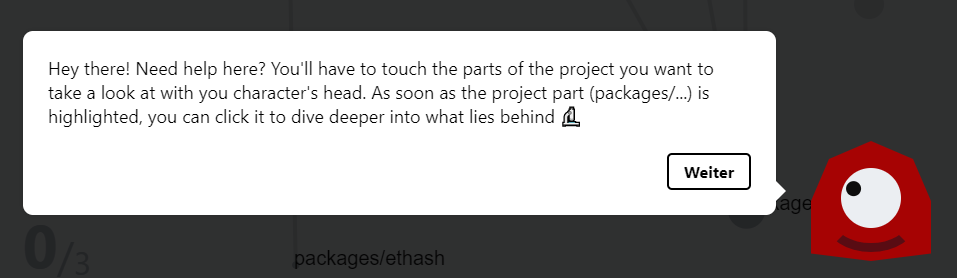
\includegraphics[width=\textwidth]{companionmessage.png}
  \caption{Helper companion within the technology probe}
  \label{fig:companion}
\end{figure}

Within that figure, attempts on making the companion having more personality are also visible. The companion's pupil follows the player's cursor to make it feel more connected to the player's actions for example. In addition to that the companion should be seem more approachable with the friendly facial features, as well as the usage of a friendly tone of text together with the usage of emoticons. If these attributes actually achieve the goal of a companion with personality, is subject to discussion based on the probing results. For the implementation details of the companion, as well as the full set of companion messages, refer to the probe codebase\footnote{See suppl. repository at path: \texttt{./technology-probe/src/ui/companion.ts}}\footnote{See suppl. repository at path: \texttt{./technology-probe/src/ui/intro.ts}}\footnote{See suppl. repository at path: \texttt{./technology-probe/src/scenes/DetailScene.ts}}.

This concludes the user-facing implementation of the technology probe. The actual generation and size of the scenes as well as the game objects is based on the underlying project's metadata and source code. How the data is programmatically read, what data is used and how it is integrated into the technology probe, is therefore subject of discussion within the next chapter.

\subsubsection{Game World Generation}

In order to generate a game world from a project's source code and metadata multiple distinct levels of tasks are necessary. To be more specific, at first the data that is needed to generate the world has to be defined, based on what outcomes are wished for and what the underlying data can provide. After that, based on the desired data, the location of that data (or the raw data necessary to then aggregate what is needed) has to be identified. The data can then be programmatically fetched from these locations and aggregated into a format that the web page containing the user-facing parts can handle. Based on that data, ultimately the game world as well as the objects in it can be generated.

% 1. Decide on which data is needed, based on the final implementation

As described, the first step to take, is to clarify which data is needed. The most important question to answer here, is: What is the desired outcome? In the case of this technology probe, the data is needed to generate game objects and the overall game world of the technology probe. Therefore it has to have properties that make it usable for such a generation, like a numeric value that can be used to generate a game object with a distinct size. Additionally contextual information important for the newcomers can be shown in the mentioned info messages. Based on these constraints the data needed for the different applications throughout the probe is aggregated in \textit{Table \ref{tab:probe-data}}.

\begin{table}[h]
  \begin{tabularx}{\textwidth}{| X | X |}
    \hline
    \textbf{Application}                                   & \textbf{Data Needed}                                                                                      \\ \hline
    (1) Subproject Objects (\textit{Overview Scene})       & Name, Size \& Connections to other subprojects                                                            \\ \hline
    (2) Discoverable Objects (\textit{Detail Scene})       & Size of the object                                                                                        \\ \hline
    (3) Contributor Messages (\textit{Detail Scene})       & (User-)Name, Link to \textit{Github} profile, Last activities within the project, Number of contributions \\ \hline
    (4) 3rd-party Package Messages (\textit{Detail Scene}) & Name, Version Number, Link to package website                                                             \\ \hline
    (5) Potential Issue Messages (\textit{Detail Scene})   & Type of Issue, Issue Location, Link to Issue Location, Size of the Issue                                  \\ \hline
  \end{tabularx}
  \caption{\label{tab:probe-data}Data needed to generate the technology probe game world}
\end{table}

In order to match the contextual information to the in-game world, the size should match the size of the respective subprojects or potential issues. As there is no directly readable size attribute, an estimation of the size in relation to the other subprojects and issues has to be found. Concerning the subprojects the most evident correlation would be to the disk space occupied by respective directory. Concerning the contextual information, some of it can be read directly from the \verb|package.json| files within the subprojects where \textit{Node.js} projects store information about all of the dependencies, both within the monorepo and to 3rd-party packages. Other information, like contributor profiles or their last activities in contrast have to be requested from \textit{Github}.

Thus, the data can be collected from the following locations. Concerning \textit{application (1)} (refer to \textit{Table \ref{tab:probe-data}} for these applications), the name of the subproject as well as its occupied disk space (=size) and the connections to other subprojects can be read directly from their respective \verb|package.json| file. A \verb|package.json| file does have a standardized schema and includes all 3rd-party packages used in two properties, called \verb|dependencies| and \verb|devDependencies|. Connections within the monorepo are also contained within those properties and marked with a prefix (in this case \verb|@ethereumjs/|).

For application (2) the only attribute needed is its size, as the discoverable objects are randomly placed in the \textit{detail scenes} and are not discernible by type. The size itself depends on the type of object, though, as contributors do have other attributes than 3rd-party-packages for example. Therefore, the size of the respective shape has to be generated based on a different data attribute.

Regarding the objects based on contributors (application (3)), this is going to be the number of contributions, as it is an easily accessible number, available through the \textit{Github \gls{api}}\footnote{\url{https://docs.github.com/en/rest}, accessed on 14th of August 2021}. Further, it also is comparable between the different types of contributors and increases the visual weight of the most important contributors. The other data points needed (name, link to profile, last activities) can also be easily fetched from the aforementioned \textit{Github \gls{api}}.

Concerning application (4), the 3rd-party-package information messages, the data for the package name and currently installed version can be sourced directly from the respective \verb|package.json|. The link to the package website is not as easy to uncover, as it is not documented within the project itself. As a workaround, the link to the package subsite within the \gls{npm} ecosystem is created through combining the package name with the base \gls{url} of the \gls{npm} website\footnote{https://www.npmjs.com/package/PACKAGE\_NAME}.

Lastly the data concerning application (5) has to be collected and aggregated into what is needed. To do this, a certain type of issue has to be decided upon. There are multiple possible issues especially in large codebases. In order to keep implementation efforts at a manageable level, only one kind of issue is going to be scanned for in the project. A possible issue, that is easly discoverable from the source project's files alone, are large files. While not necessarily directly connected to badly written code, such large files can be hard to understand and messy \cite{so2012large} for newcomers. Therefore, the identification of such files could present an angle for communication with existing contributors, or creating issues for possible refactoring within the source project's repository -- possibly as way to introduce themselves into a project. With the choice on the type of issue out of the way, the needed data (file location, link to the file location and the size of the file) can be gathered directly from the underlying project.

After clarifying, where the data that is needed can be collected from, the actual collection has to happen. Based on the clarification there are two distinct locations, where data has to be fetched from. Firstly, the codebase's files and directories and secondly \textit{Github's public \gls{api}}. The simplest way to access that information is, to do it locally through a script, that programmatically reads from the file system and accesses the necessary \gls{api}. To stay in the \textit{Javascript} ecosystem, the script is created with \textit{Node.js} and can be found within the technology probe's source code as well\footnote{See suppl. repository at path: \texttt{./technology-probe/scripts/get-metadata.js}}. This script can be executed manually and produces an output file containing all the necessary information needed to generate the game world. This file can also be found in the same repository\footnote{See suppl. repository at path: \texttt{./technology-probe/metadata/project.json}}. This file contains all of that information in a file format (.json) readable by the technology probe's source code, in a format that can be easily used for generating the game world. It includes data that is already aggregated into a format that can be used as-is to generate all the game objects, including the size of the shapes, the textual content shown in the info messages, and the links necessary to lead the player to the actual contributors, packages, and more. This is then directly used within the context of the webpage to generate the game objects. Again, the implementation details can be found in the respective repository\footnote{see page 4 for the accompanying repository URL}.

\subsection{Data Collection}

In addition to the user-facing implementation and the creation of the game world, user-generated data has to be collected. This can then be used to draw conclusions from the probe as a whole and to ultimately answer the research questions. As already mentioned in the methodology chapter, user-generated data is collected in four different ways: \textbf{Capturing demographic information (1), logging participant interactions (2), questions on the underyling project (3) \& questions on the research topic (4)}. For all of these ways, the specific questions -- or logging events for that matter -- have to be defined and implemented.

Starting with the demographic information, this should just give some additional contextual information to the participant's background. The primary goal is to research how developers experience playful elements in software development projects unbeknownst to them. Thus, questions on the professional background of the participants are crucial. The participants are also given the option to give their name and age, if they so desire. That concludes the small set of demographic questions to be asked. As said, these are just to give some additional context for the result argumentation and to make sure that the participant is part of the target group. Because there are not going to be any generalizeable or representative conclusions, no additional demographic information is asked for. The final set of input from the participant at this stage is presented in \textit{Appendix \ref{append:collect}}.

Regarding the second way of collecting data -- logging user interactions within the probe -- additional considerations have to be made. More specifically, the types of the interactions have to be considered and how they are actually logged within the probe. Firstly, a structure has to be defined on how the single events are logged and distinguish the events from each other. The distinction itself is done through a pre-defined two-character code, so that it can easily be aggregated and analyzed if needed. The full table of all the codes used throughout the probe can be found in \textit{Appendix \ref{append:collect-log}}. To give context to the singular events, when logging these, timestamps are included to keep track of when and in what sequence these events happened. Additionally, there is the possibility to add custom text to these events if so needed. Within the probe's codebase a function was the created (see the respective file for the implementation details\footnote{Source code file within the accompanying repository at: \texttt{./technology-probe/src/logger.ts}}, making it possible to track events from within the code. These are then persisted through Google's Firebase \footnote{\url{https://firebase.google.com/}, accessed on 14th of August 2021} service, where for each participant the answers to all questions and the logged events are stored for later analysis.

The third way of collecting data, is concerned with getting a sense on how the data about the project translated into the participant's understanding of those. Therefore, it should consist of question on what was presented regarding the underlying projects. These questions were based on the metadata collected for the generation of the game world and directly target what was presented. The final set of questions can be found in \textit{Appendix \ref{append:collect}}. Question (1) is about how vividly the participant remembers the contributors shown, as they are the prime social links of a project. Question (2) is added as a way of finding out if the participants connected the subproject size to the size of the shape displayed in the overview scene. The next question (3) is included as a way to find out if the participant recognizes what the lines between the subproject game objects are trying to visualize and how memorable the overall visualization in the \textit{overview scene} was. Question (4) targets the 3rd-party-packages and if the participant remembers some of the ones that were discovered. The last question (5) is targeted towards how participants viewed the last kind of revealable information, the large files that were identified within the game world generation procedure. This last question also includes the participant's opinion on how they would rate the issue of these large files in terms of graveness of the issue. While this answer is not strictly confined to the underlying project it is very much connected to the topic of the question. Additionally, it transitions into the questions on the research topic as a whole.

These questions on the overall research topic are also included in \textit{Appendix \ref{append:collect}}. In the following, for each of the questions a reasoning is given on why it was included. Question (1) tries to investigate if the participants themselves subjectively feel like they have learnt something on the underlying project. To make sure to get more than just a positive or negative reply, within the question it is explicitly mentioned, that the participant should give an answer on what was learned. Additionally, if the participant did not feel like something was learned, an explicit enquiry to what should have been included is added to the question.

Question (2) tries to expand from the learning or onboarding aspect into the overall subjective experience of the participant exposed to the probe. The question is asked in an open-ended manner in order to get qualitative data based on the participant's experiences throughout the probe. Specifically mentioning parts that were liked or disliked by the participant is also encouraged through the wording of the question.

The following question (3) focuses on a single feature of the probe, that might be of value also in contexts other than the technology probe -- the companion and how the participant experienced it. It also acknowledges that the companion might only have been visible as a status indicator not as a helping feature.

Question (4) opens up again, more towards how the participants would describe their stance towards an interactive visualization (as is the case with this technology probe) for software development onboarding purposes. Additionally, it asks for input on projects that might be adequate for such visualizations and on which projects the participant would want to try them out. For, if the participant expresses that they cannot imagine themselves using something like that, a direct query on what they would use instead is included.

Question (5) completely moves away from playful elements in onboarding and tries to get a personal perspective on how each of the participants usually approach onboarding. Specific cues are given to give the participants a clue on what interesting elements of the onboarding process are.

The question after (6) then is more of an optional question, targeted at developers working on open source projects specifically. As the onboarding in such projects is different from a local on-site team, it is included as a way to gather information about how the nature of the project changes how an onboarding process is done at a personal level.

Question (7) then focuses on the explorative nature of the research done within this thesis. It tries to gather input from the \textit{experts} on the topic, the developers, the participants on how they would integrate playful elements in an onboarding context.

Question (8) builds upon that an asks for two things. Firstly, the general stance towards the usage of playful elements in onboarding processes in order to gather information about developers stance towards playfulness in their work environment. Secondly, the nature of the project is also included as a way to gather data on how participants would perceive playful elements in different contexts (namely working on open source software vs. commercial products).

In the last formulated question (9) the participants are asked for game mechanics familiar to them, that they would deem valuable as playful elements in onboarding processes. While this is a larger task for the participants, input on that question is very valuable, as it further explores ways of using play and playfulness in onboarding contexts.

Finally, question (10) is included as a space, where the participants can give additional feedback independently of the preceding questions.

Overall, all the questions are open-ended where possible, to gather as much qualitative input as possible. Due to the asynchronous and remote nature of the probe, there is no possibility to immediately query the participant on what was said before, though. Due to this downside of the approach, these queries are included within the question, where possible. Concerning the technical implementation, the questions are logged to \textit{Firebase} and added to the participant's data, together with the demographic data and logged events. How the questions are included within the technology probe as a whole is laid out in detail in chapter 4.6.

\subsection{Participant Selection}

After clarifying how the technology probe is implemented, how the game world is generated and how the qualitative data is gathered only two aspects of the probe are left before the study can be executed. Firstly, all of the single parts of the technology probe have to be put into a distinct sequence, so that the participants are introduced to the study, can give their consent, go through the probe and finally answer the questions outlined before. This is going to be outlined in the next chapter. Secondly, that sequence has to be gone through by a set of participants, that have to be selected based on a set of requirements.

The single most important requirement is that the probe is executed by participants that are part of the context that should be investigated. In this case, these are software developers of any kind. There is no need to limit the selected participants to a certain group or level of experience, as the topic of onboarding is something every kind of developer is exposed to some degree. On the contrary, to get a wide variety of different responses it is beneficial to have a very diverse set of participants (concerning age, experience, and more). Thus, the only requirement concerning the participants is going to be that they are software developers, either professionally, on a leisurely basis or nascent ones just starting out in the field. As the study is going to be held remotely and asynchronously, the participants do not have to agree onto a fixed data and time, but can choose for themselves when they want to take part within the probe.

Concerning the number of participants needed, there is no definite amount of participants needed to reach a representative conclusion. Rather, the number of participants should be enough, that an amount of data is generated that produces a big enough foundation to answer the research questions. This is not tied to a set number of participants, but to the data generated by each participant. To get answers that are diverse enough, a minimum number of participants should be set -- in this case five developers. If, after reaching that number of participants in the probe, not enough data to draw conclusions from is generated, additional participants are going to be asked to take part in the study.

\subsection{The Final Technology Probe}

At this point every part of the probe, the constraints around it and the desired participants are defined. As mentioned before, the only step left at this point is to create a coherent probe that includes all of the carefully created parts in a structured manner. To recapitulate, these parts are: \textbf{An introduction to the study, a consent and data protection form, the interactive visualization of the \textit{@etherumjs} project, the demographic questions, the questions on the underlying project \& the questions on the research topic}. All of that has to be combined into an easily accessible technology probe accessible through a browser on a webpage. Together with introductory messages and further information for the participant, the final structure of the probe is as follows:

\begin{enumerate}
  \item{Introduction message to inform the participant on the study, the goal of the study, and the overall procedure}
  \item{Consent \& Data Protection to follow the research ethics guidelines}
  \item{Demographic questions}
  \item{An introduction to the interactive part of the probe}
  \item{Beginning of the interactive part within the probe overview scene}
  \item{Revealing important parts of the project within the probe detail scenes}
  \item{Questions on the underlying project}
  \item{Questions on the research topic}
  \item{Outro message}
\end{enumerate}

For all of these steps a seperate subpage has been created that can be seen in detail in \textit{Appendix \ref{append:probe-steps}}. The implementation of the view logic to cycle through these steps and the elements and styles of these subpages has been done outside of the interactive \textit{p5.js} application with just \textit{\gls{html}, \gls{css}}, and \textit{Javascript (Typescript)}. Details of the implementation can be found mainly in the two respective files of the technology probe codebase\footnote{See suppl. repository at path: \texttt{./technology-probe/src/ui/intro.ts}}\footnote{See suppl. repository at path: \texttt{./technology-probe/index.html}}\footnote{See suppl. repository at path: \texttt{./technology-probe/styles.scss}}. The companion, that was described in detail in chapter 4.3.1 is ultimately included on the lower right of the interactive part of the probe. In addition to that, a counter was added to the technology probe steps 5 \& 6, so that participants get a sense of their progress within the probes. Additionally, the exploration of the subprojects is limited to three, to limit the amount of time needed to complete these steps of the probe. This concludes the documentation of the design and implementation of the research done within this thesis. The next chapter now focuses on the results \& conclusions drawn from that research.
